\section{Tutorial -- Flowsheets with Recycle}

This section provides a tutorial on working with flowsheets containing recycle. Sections \ref{tutorial.simple.flow} and \ref{tutorial.sim.flowsheet} provide tutorials for creating flowsheets, in this section a pre-constructed flowsheet is used.

\begin{enumerate}
	\item From the example files, copy the Recycle\bs Mass\_Bal\_Test\_02.foqus example file to a convenient location (see Section \ref{tutorial.example.files}).
	\item Open FOQUS.
\end{enumerate}
\begin{samepage}\begin{enumerate}
	\setcounter{enumi}{2}
	\item Open the Mass\_Bal\_Test\_02.foqus file.
	\begin{enumerate}
		\item Open the \textbf{\underline{Session}} drop-down menu on the right side of the \textbf{\underline{Session}} button (Figure \ref{fig.recycle.tut1}).
		\item Select \bu{Open Session} from the drop-down menu.
		\item Locate Mass\_Bal\_Test\_02.foqus in the file browser, and open it.
	\end{enumerate}
	\setcounter{enumi}{3}
	\item Click \bu{Flowsheet} button from the toolbar at the top of the Home window.
\end{enumerate}\end{samepage}

The flowsheet is shown in Figure \ref{fig.recycle.tut1}.  The flowsheet consists of two reactors in recycle loops.  The flowsheet contains mixers, reactors, separators, and splitters. Each node uses a set of simple calculations in the node script section. The tear edges are shown in light blue.

\begin{figure}[H]
	\begin{center}
		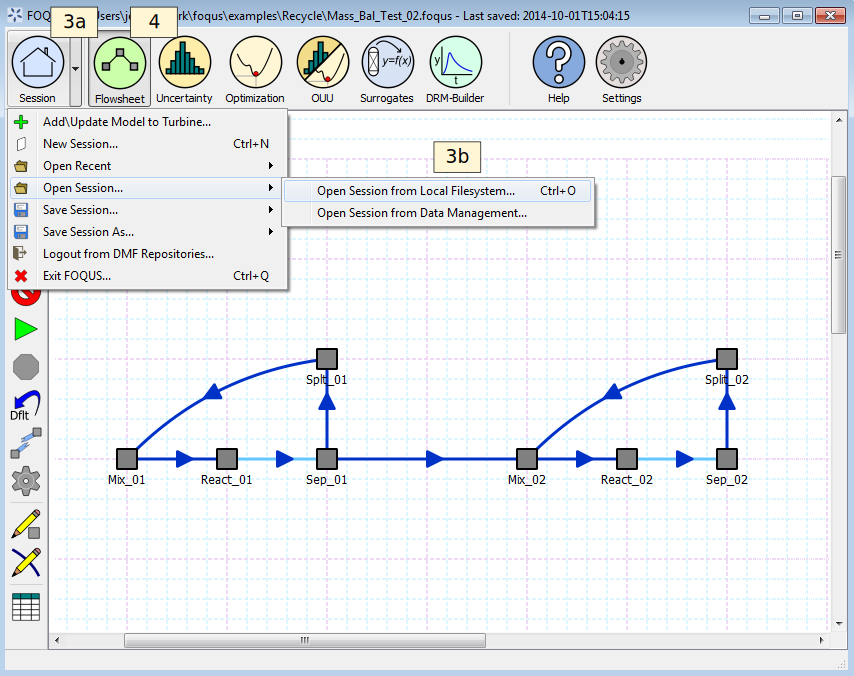
\includegraphics[scale=0.55]{Chapt_flowsheet/figs/recycle_tut1}
		\caption{Flowsheet with Recycle}
		\label{fig.recycle.tut1}
	\end{center}
\end{figure}

\begin{enumerate}
	\setcounter{enumi}{4}
	\item Inspect a node.
	\begin{enumerate}
		\item Make sure the Selection tool is selected  (Figure \ref{fig.recycle.tut2}).
		\item Open the Node Editor by clicking the \textbf{\underline{Node Edit}} button in the left toolbar in the Flowsheet view.
		\item Click the ``React\_01'' node.
		\item Click \bu{Input Variables} table. Note: Some input rows are colored red. This denotes that their values are set by output of the previous flowsheet node by the edge connecting ``Mix\_01'' to ``React\_01.''
		\item Click the \bu{Node Script} tab.
		\item Note the equations. \textbf{\underline{Input Variables}} are stored in the x dictionary and \textbf{\underline{Output Variables}} are stored in the f dictionary.
	\end{enumerate}
	\item Click the gear icon in the left toolbar (see Figure \ref{fig.recycle.tut2}).  The tear solver settings are shown in Figure \ref{fig.tear.settings}.
\end{enumerate}
	
\begin{figure}[H]
	\begin{center}
		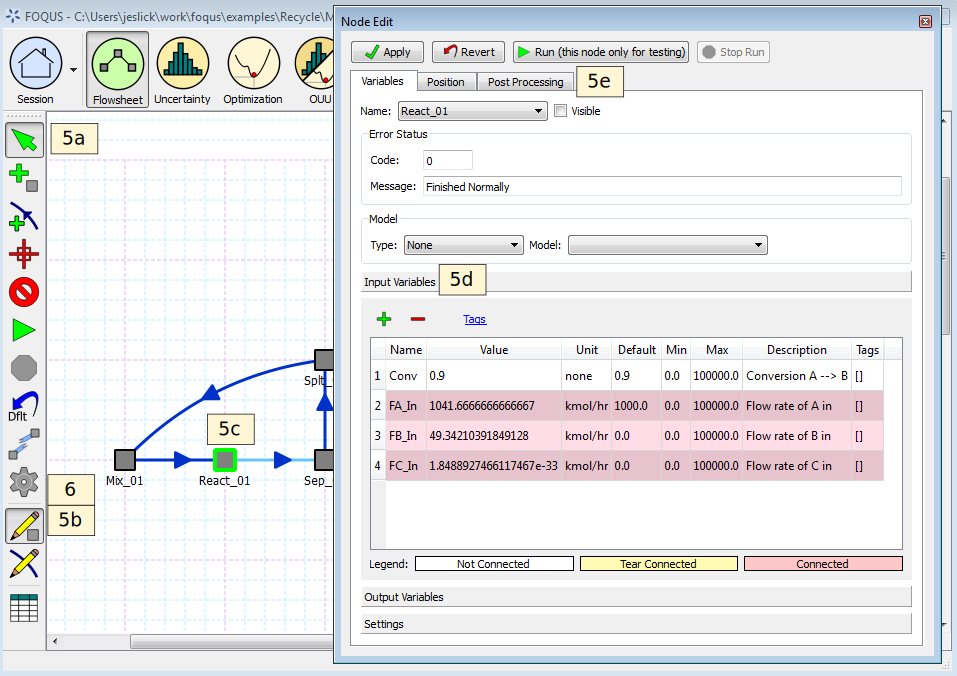
\includegraphics[scale=0.55]{Chapt_flowsheet/figs/recycle_tut2}
		\caption{React\_01 Node}
		\label{fig.recycle.tut2}
	\end{center}
\end{figure}

\begin{figure}[H]
	\begin{center}
		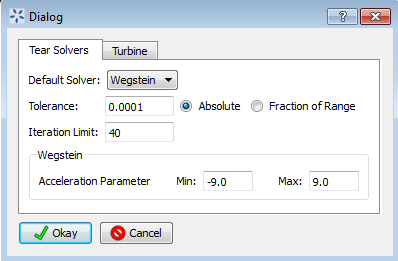
\includegraphics[scale=0.55]{Chapt_flowsheet/figs/tear_solver_settings}
		\caption{Tear Solver Settings}
		\label{fig.tear.settings}
	\end{center}
\end{figure}

\begin{samepage}
\begin{enumerate}
	\setcounter{enumi}{6}
	\item Remove the tear edges.
	\begin{enumerate}
		\item Close the Node Editor.
		\item Open the Edge Editor. Click the \bu{Edge Editor} icon in the left toolbar (see Figure \ref{fig.recycle.tut3}).
		\item Click the edge between ``React\_01'' and ``Sep\_01.''
		\item In the Edge Editor, clear the \bu{Tear} checkbox.
		\item Repeat for the other tear edge.
	\end{enumerate}
	\item Close the Edge Editor.
\end{enumerate}
\end{samepage}

\begin{figure}[H]
	\begin{center}
		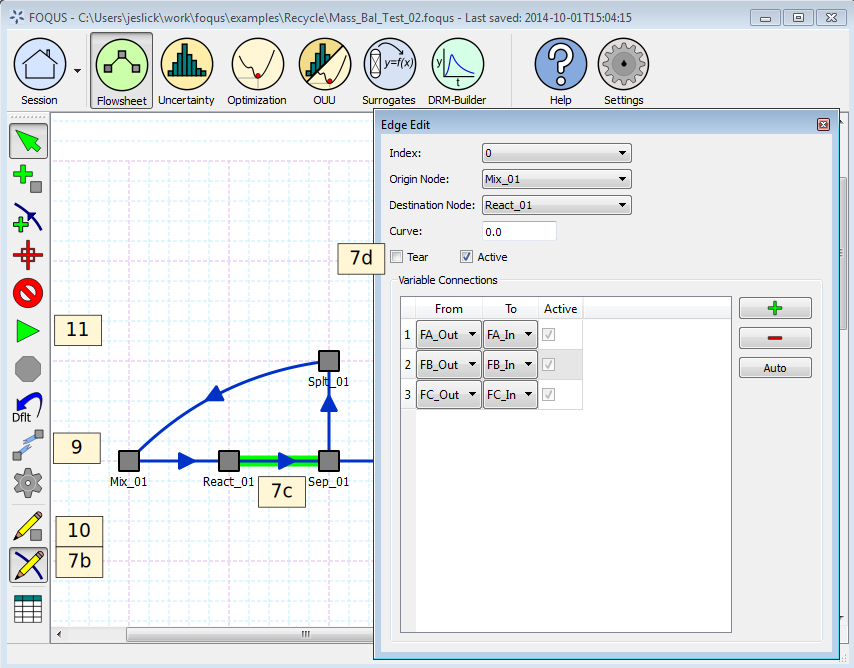
\includegraphics[scale=0.55]{Chapt_flowsheet/figs/recycle_tut3}
		\caption{Edge Edit}
		\label{fig.recycle.tut3}
	\end{center}
\end{figure}

There should now be no tear edges in the flowsheet. The user can select tear edges or FOQUS can automatically select a set. If there is not a valid set of tear edges marked when a flowsheet is run, tear edges will automatically be selected.
\begin{enumerate}
	\setcounter{enumi}{8}
	\item Automatically select a tear edge set by clicking the \bu{Tear} icon in the left toolbar (see Figure \ref{fig.recycle.tut3}).
	\item Open the Node Editor and look at node ``Sep\_01.''  In the Input Variables table, notice that some of the input lines are colored yellow. The yellow inputs serve as initial guesses for the tear solver. The final value will be different from the initial value.
	\item Click the \textbf{\underline{Run}} button on the left toolbar.  The flowsheet should solve quickly.
	\item The results of the completed run are in the flowsheet.  An entry will also be created in the Flowsheet Results data table (see Section \ref{tutorials.fs.data}).
\end{enumerate}

